\documentclass[10pt]{article}
\usepackage[T1]{fontenc}
\usepackage[utf8]{inputenc}
\usepackage{microtype}
\usepackage{graphicx}
\usepackage{booktabs}
\usepackage{tabularx}
\usepackage{array}
\usepackage{amsmath,amssymb}
\usepackage{xcolor}
\usepackage{cite}
\usepackage{hyperref}
\usepackage[nameinlink,noabbrev]{cleveref}
\usepackage{placeins}

\definecolor{linkblue}{HTML}{245B8A}
\hypersetup{
  colorlinks=true,
  linkcolor=linkblue,
  citecolor=linkblue,
  urlcolor=linkblue,
  pdfauthor={Adit Patil},
  pdftitle={Bundle Neural Networks for Functional Connectomes}
}

\graphicspath{{generated/figures/}}
\interdisplaylinepenalty=2500
\hyphenation{con-nec-tome con-nec-tomes over-smooth-ing}

\newcommand{\ASD}{autism spectrum disorder}
\newcommand{\ABIDE}{Autism Brain Imaging Data Exchange}
\newcommand{\BuNN}{Bundle Neural Network}
\newcommand{\GCN}{Graph Convolutional Network}
\newcommand{\FC}{functional connectivity}
\newcommand{\BA}{balanced accuracy}
\newcommand{\code}[1]{\texttt{#1}}
% Generated by scripts/build_manuscript_inputs.py; do not edit manually.
\providecommand{\StudyParentRows}{769}
\providecommand{\StudyTechnicalExclusions}{15}
\providecommand{\StudyParticipants}{754}
\providecommand{\StudySites}{18}
\providecommand{\StudyASD}{371}
\providecommand{\StudyControls}{383}
\providecommand{\StudyROIs}{116}
\providecommand{\StudyEdges}{6,670}
\providecommand{\CovariatesBA}{0.5652}
\providecommand{\ConnectomeBA}{0.6401}
\providecommand{\CombinedBA}{0.6336}
\providecommand{\BunnGcnEstimate}{-0.00958}
\providecommand{\BunnGcnCILow}{-0.03665}
\providecommand{\BunnGcnCIHigh}{0.01146}
\providecommand{\BunnGcnP}{0.524}
\providecommand{\PracticalMargin}{0.03}
\providecommand{\BunnElasticEstimate}{-0.05516}
\providecommand{\BunnElasticCILow}{-0.08297}
\providecommand{\BunnElasticCIHigh}{-0.02752}
\providecommand{\BunnElasticP}{0.0018}
\providecommand{\RankEstimate}{-0.00719}
\providecommand{\RankCILow}{-0.01310}
\providecommand{\RankCIHigh}{-0.00105}
\providecommand{\LeaveOneSitePositive}{1}
\providecommand{\SeedPositive}{2}
\providecommand{\FavorableIntervals}{0}
\providecommand{\UnfavorableSeedIntervals}{1}
\providecommand{\GcnParameters}{5,889}
\providecommand{\BunnParameters}{8,529}
\providecommand{\GcnFitHours}{15.09}
\providecommand{\BunnFitHours}{31.14}
\providecommand{\GcnCurveBA}{0.5945}
\providecommand{\BunnCurveBA}{0.5849}


\hypersetup{pdftitle={Supplementary Material: Bundle Neural Networks for Functional Connectomes}}
\renewcommand{\thefigure}{S\arabic{figure}}
\renewcommand{\thetable}{S\arabic{table}}

\title{Supplementary Material\\
\large Bundle Neural Networks for Functional Connectomes}
\author{Adit Patil\\
\small School of Scholars, Akola, India}
\date{}

\begin{document}
\maketitle

\section{Frozen analysis contract}

The manuscript is compiled from the frozen Step 13 evidence package. The
contract binds the claim ledger, result snapshot, artifact manifest, and paper
asset manifest by SHA-256 digest. The manuscript-input builder refuses to
generate tables or numeric macros if any bound input has changed. This
supplement reports pre-specified secondary summaries; it introduces no new
model fitting, participant exclusions, hyperparameter selection, or
confirmatory inference.

The claim boundary is deliberately narrow. Results apply to the analyzed
ABIDE-I C-PAC filtered, no-global-signal-regression, AAL-116 pipeline with
positive-edge graphs and connectivity-profile node features. They do not
establish clinical utility, anatomical or causal connectivity, biological
bundle geometry, or universal inferiority of BuNNs.

\section{Representation endpoints}

Raw learned-BuNN embeddings can occupy node-specific frames. Cross-node
diagnostics were therefore computed only after mapping embeddings into a
common learned frame. The primary endpoint was normalized effective rank at
layer 2, compared using each operator's matched density-zero anchor.
Dispersion, cosine similarity, invariant edge-transport distance, and
encoder-to-layer-2 rank change were secondary diagnostics.

\begin{table}[H]
\centering
\caption{BuNN-minus-GCN matched-anchor representation contrasts at layer 2.}
\label{tab:supp-representation}
\footnotesize
\begin{tabularx}{\textwidth}{Xrr}
\toprule
Endpoint & Estimate & 95\% site-bootstrap CI \\
\midrule
Normalized effective rank & -0.0072 & [-0.0131, -0.0010] \\
Normalized dispersion & -0.0417 & [-0.0523, -0.0306] \\
Mean pairwise cosine similarity & 0.0415 & [0.0319, 0.0507] \\
Invariant edge-transport distance & -0.6436 & [-0.8205, -0.4720] \\
Encoder-to-layer-2 effective-rank change & -0.0056 & [-0.0144, 0.0048] \\
\bottomrule
\end{tabularx}
\end{table}


\section{Robustness summaries}

The equal-site mean was the confirmatory aggregation because each held-out
site defined one generalization unit. Participant-weighted and site-median
summaries were pre-listed sensitivity analyses, not alternative routes to a
positive conclusion.

\begin{figure}[t]
  \centering
  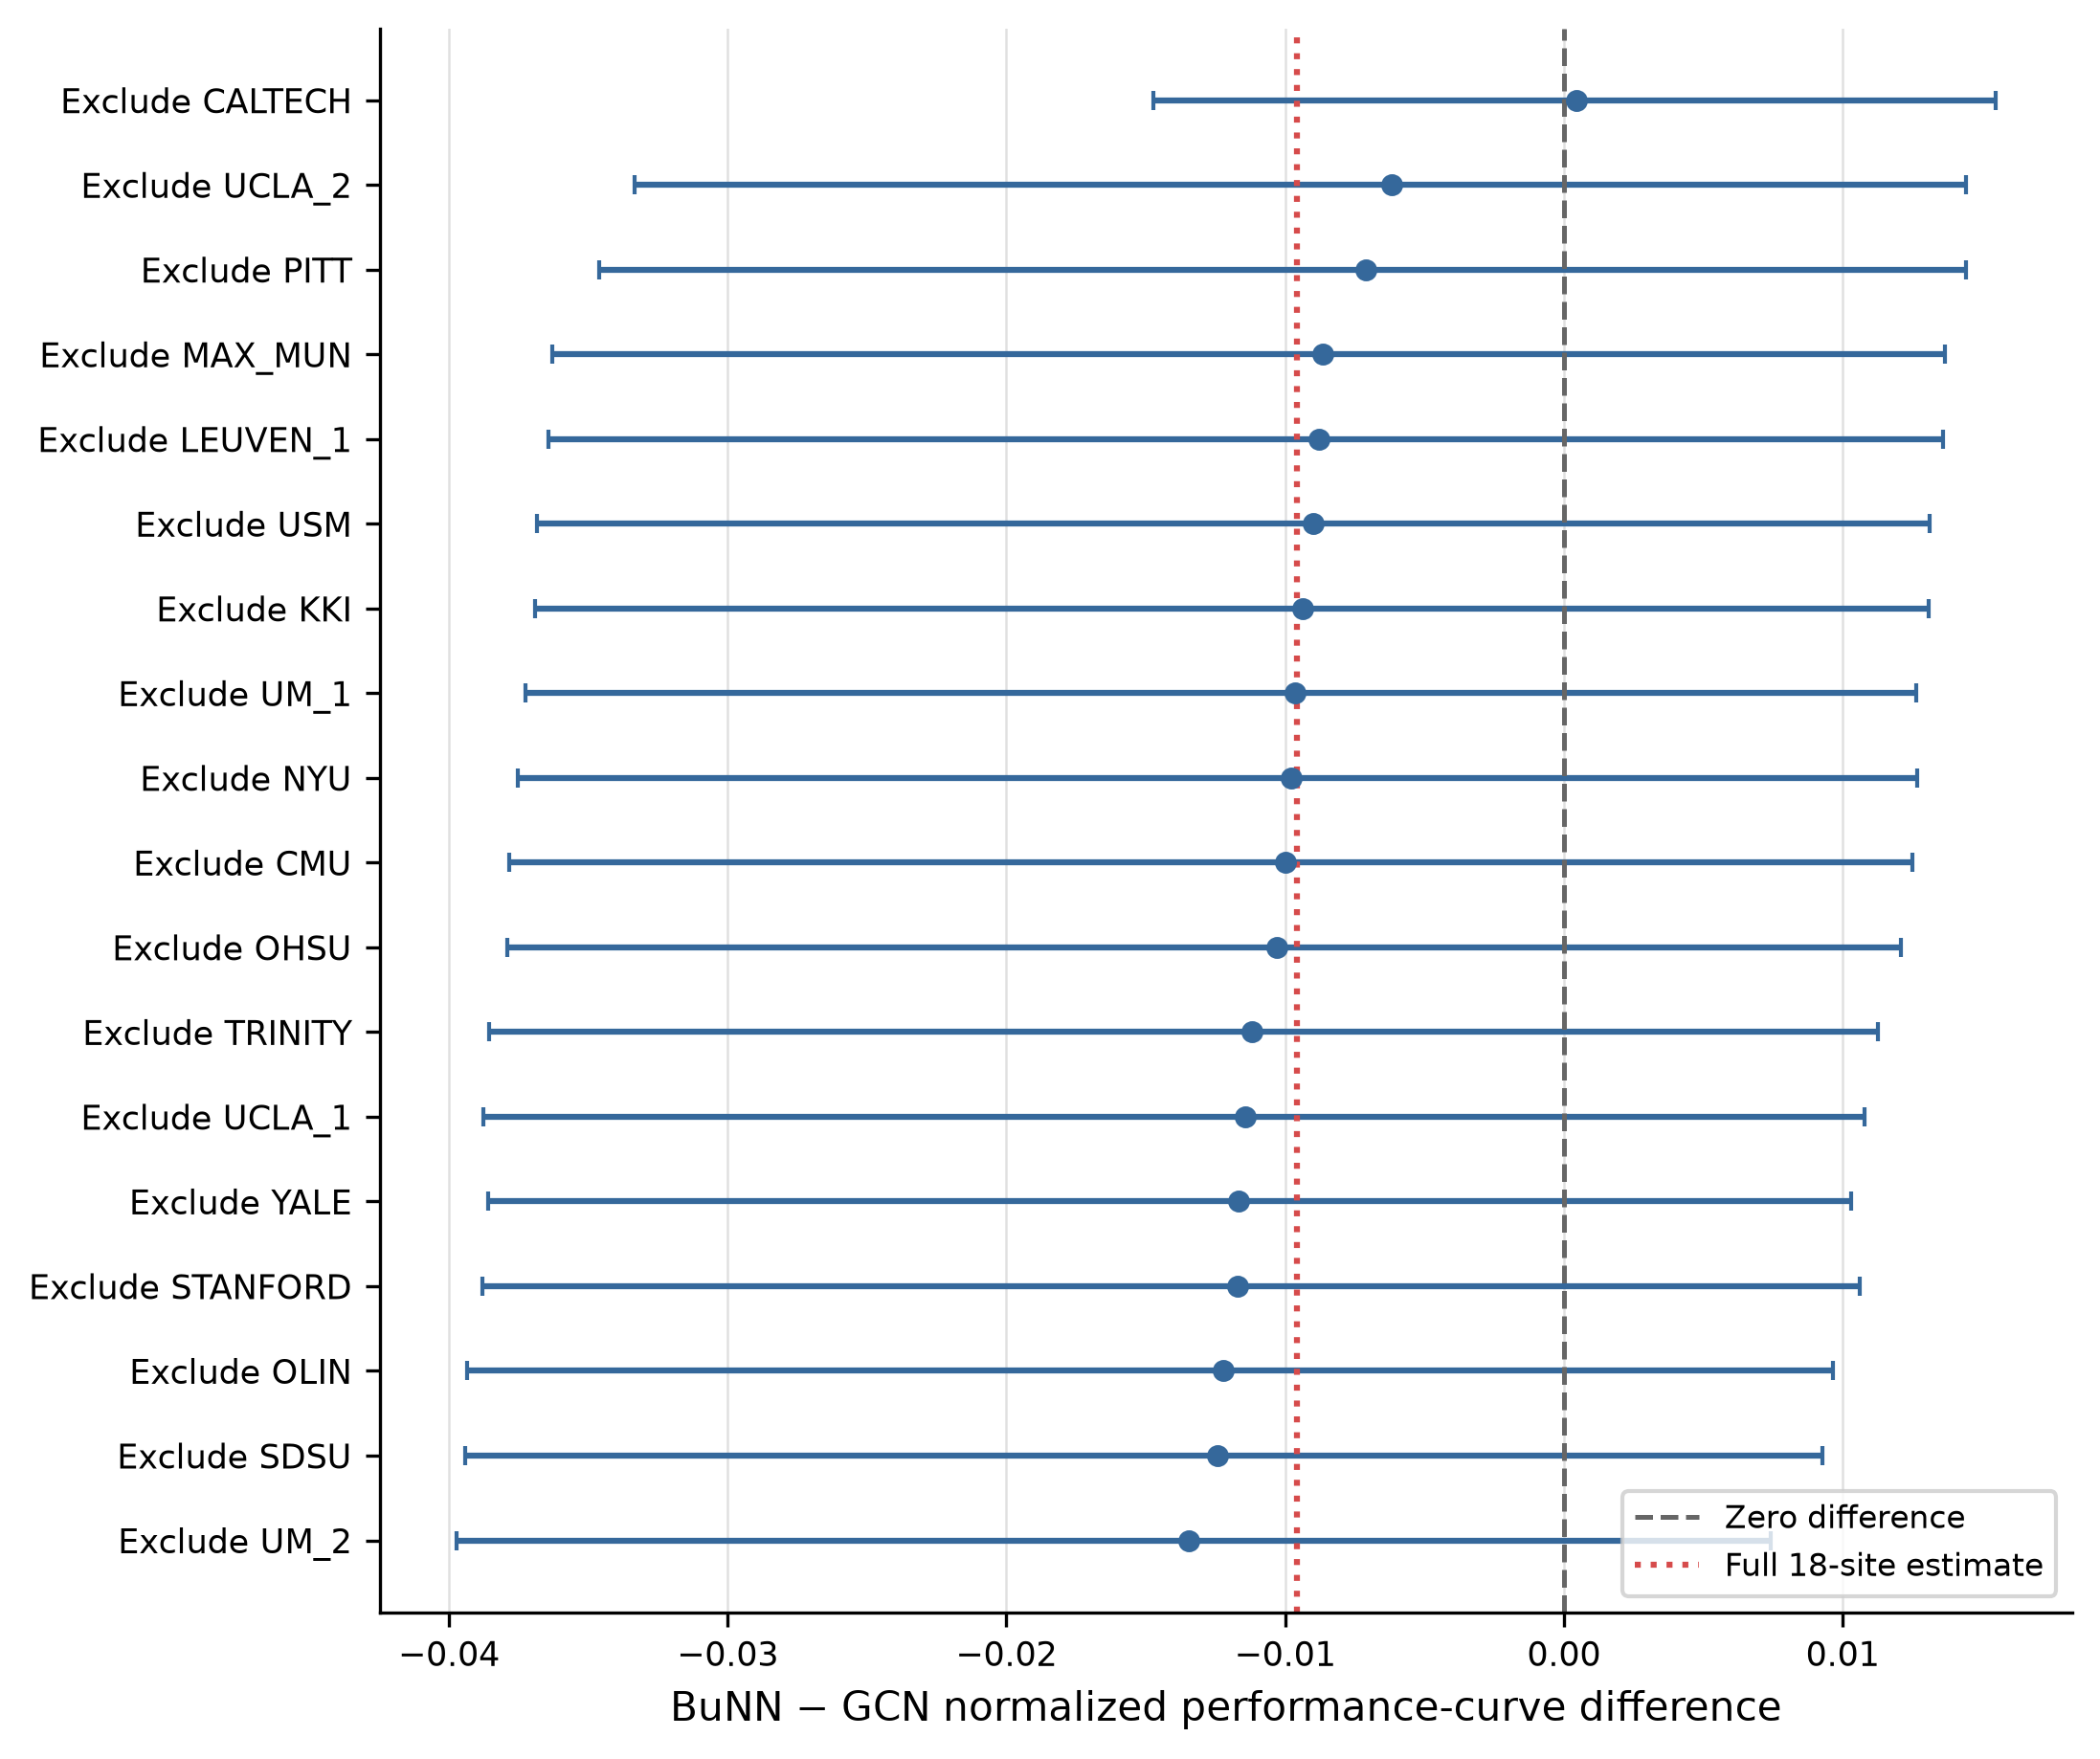
\includegraphics[width=0.86\textwidth]{site_influence.png}
  \caption{Leave-one-site-out influence analysis for the primary BuNN-minus-GCN
  curve contrast. Every pre-listed exclusion is shown.}
  \label{fig:supp-site-influence}
\end{figure}

\begin{figure}[t]
  \centering
  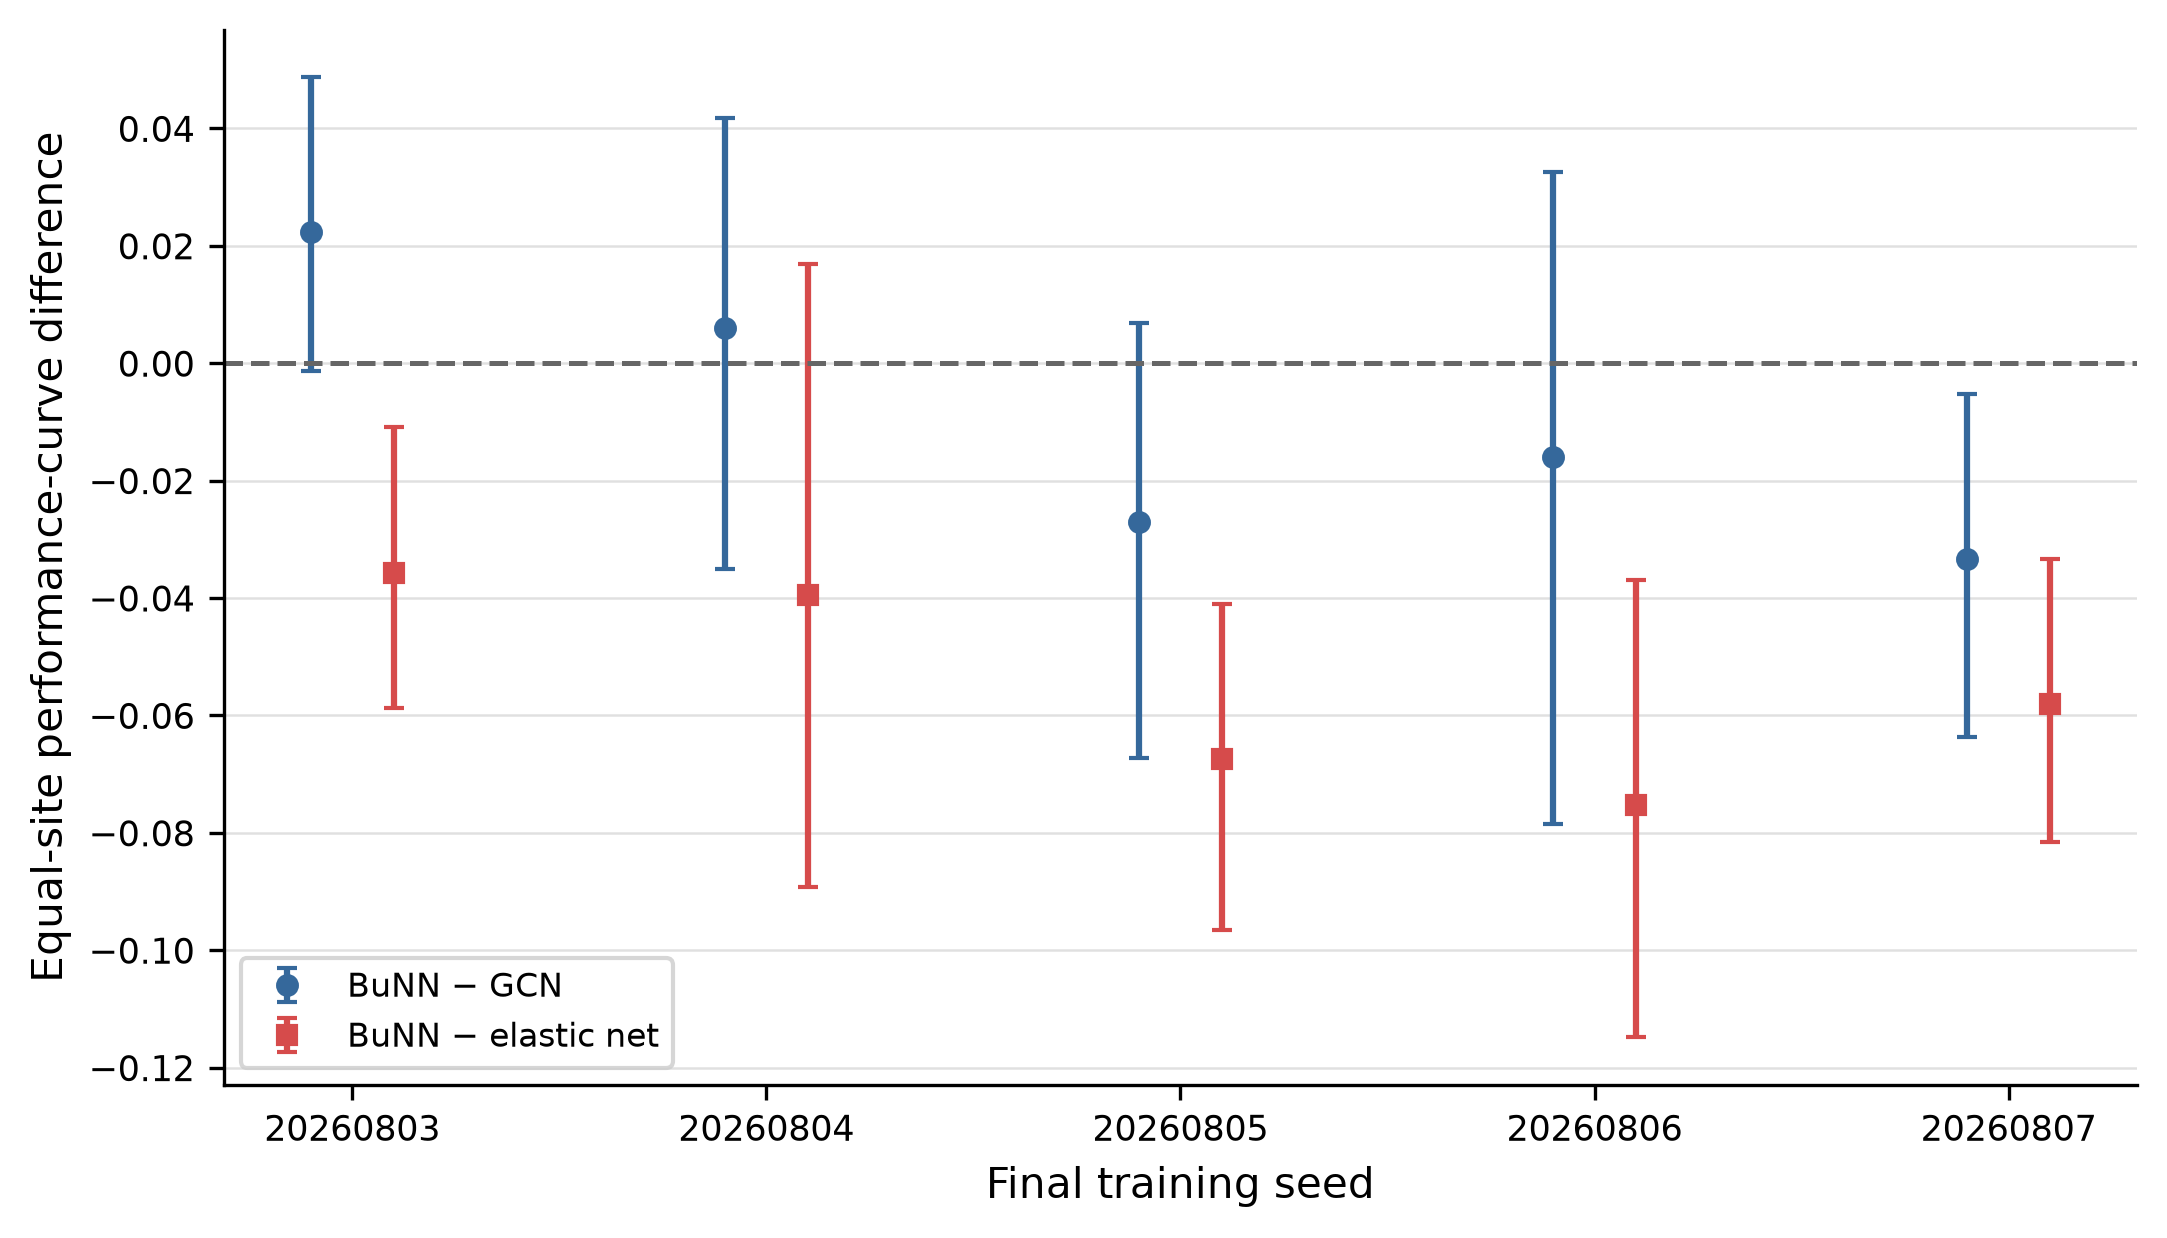
\includegraphics[width=0.78\textwidth]{seed_stability.png}
  \caption{Seed-specific curve contrasts. Intervals resample held-out sites
  within each fixed final seed. Seed-level results are robustness diagnostics,
  not alternative primary analyses.}
  \label{fig:supp-seed-stability}
\end{figure}

\FloatBarrier
\input{generated/tex/supplement_robustness_tabular.tex}
\FloatBarrier

The leave-one-site-out analysis recomputed each named contrast after excluding
one outer site at a time. Seed-specific analyses recomputed the primary curve
contrast separately for every fixed final seed. These analyses quantify site
and optimization sensitivity; they do not replace the frozen primary
estimand.

\section{Reproducibility and integrity}

The repository records the exact participant manifest, technical exclusion
rules, connectome construction, held-out-site splits, operator contracts,
tuning budgets, final seeds, source hashes, run audits, and aggregate result
artifacts. Generated manuscript values are not copied manually: the build
script reads the frozen result snapshot and writes LaTeX macros and tables.
Unit tests verify the input hashes, deterministic generation, claim coverage,
bibliography resolution, and the absence of manually duplicated primary
results in narrative source files.

\end{document}
